\documentclass[11pt,a4paper]{article}
\usepackage[utf8]{inputenc}
\usepackage[T1]{fontenc}
\usepackage[margin=1in]{geometry}
\usepackage{graphicx}
\usepackage{hyperref}
\usepackage{xcolor}
\usepackage{float}
\usepackage{listings}
\usepackage{upquote}

% Code listing style
\lstset{
    basicstyle=\ttfamily\small,
    breaklines=true,
    breakatwhitespace=false,
    frame=single,
    numbers=left,
    numberstyle=\tiny,
    backgroundcolor=\color{gray!10},
    keywordstyle=\color{blue},
    commentstyle=\color{green!50!black},
    stringstyle=\color{red},
    showstringspaces=false
}

\title{\textbf{Practice 1 - Setting up the Stretch Robot Simulator}}
\author{
    Robotics and Cyber-Physical Systems \\
    School of Sciences and Engineering \\
    Tecnol\'ogico de Monterrey
}
\date{}

\begin{document}

\maketitle

\section{Introduction}

The Hello Robot Stretch is a mobile manipulator for research and assistive robotics. This practice introduces the Stretch MuJoCo Digital Twin---a high-fidelity physics simulation for developing robotics algorithms.

\begin{figure}[H]
    \centering
    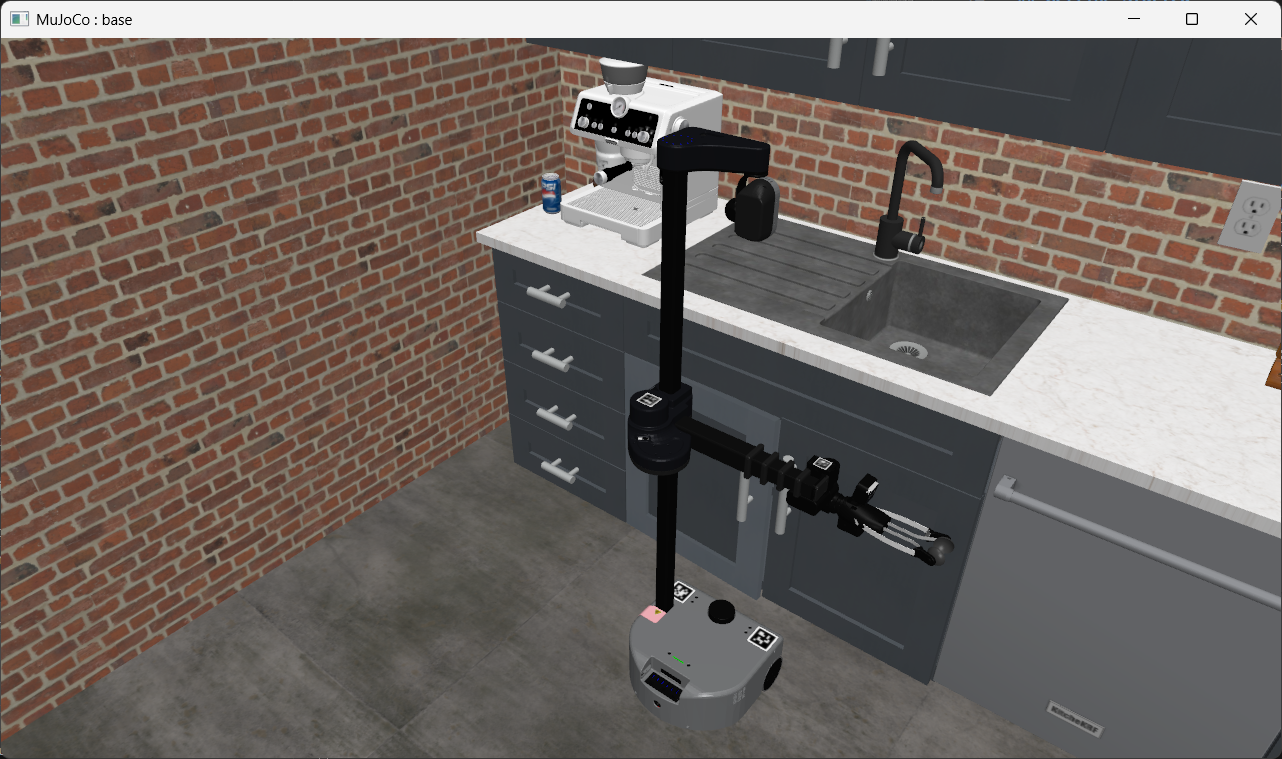
\includegraphics[width=0.5\linewidth]{stretch_robocasa.png}
    \caption{Stretch robot operating in the MuJoCo simulation environment}
    \label{fig:stretch_sim}
\end{figure}

\textbf{Objectives:}
\begin{itemize}
    \item Install and verify the base simulator
    \item Complete a block stacking challenge using teleoperation
    \item Optionally install and verify RoboCasa kitchen environments
\end{itemize}

\section{Requirements}

\begin{itemize}
    \item Windows, macOS, or Linux laptop
    \item Git
    \item \texttt{uv} package manager
    \item Code editor (VS Code recommended)
    \item \textbf{Optional:} Xbox-compatible gamepad
    \item 5+ GB free disk space
\end{itemize}

\section{Setup}

\textbf{Video Tutorial:} \url{https://youtu.be/FLPB3TQcUoI}

\subsection{Install uv Package Manager}

\textbf{Windows:}
\begin{lstlisting}[language=bash]
powershell -c "irm https://astral.sh/uv/install.ps1 | iex"
\end{lstlisting}

\textbf{macOS/Linux:}
\begin{lstlisting}[language=bash]
curl -LsSf https://astral.sh/uv/install.sh | sh
\end{lstlisting}

Restart your terminal after installation.

\subsection{Clone Repository}

\begin{lstlisting}[language=bash]
git clone https://github.com/SilentSammy/stretch_mujoco_digital_twin --recurse-submodules
cd stretch_mujoco_digital_twin
\end{lstlisting}

\textbf{Linux users:} If you get build errors, install:
\begin{lstlisting}[language=bash]
sudo apt install build-essential python3-dev linux-headers-$(uname -r)
\end{lstlisting}

\section{Part 1: Verify Base Simulation}

Run the simulator:

\begin{lstlisting}[language=bash]
uv run teleop_demo.py
\end{lstlisting}

You should see:
\begin{itemize}
    \item Terminal: \texttt{=== Running on simulation backend ===}
    \item MuJoCo viewer with Stretch robot
    \item Two colored blocks (blue box and red cylinder)
\end{itemize}

\textbf{Important:} Before controlling the robot, click away from the MuJoCo viewer (e.g., click the taskbar or another window). This prevents keyboard inputs from triggering simulator functions. The controls will still work when the window is unfocused.

\begin{figure}[H]
    \centering
    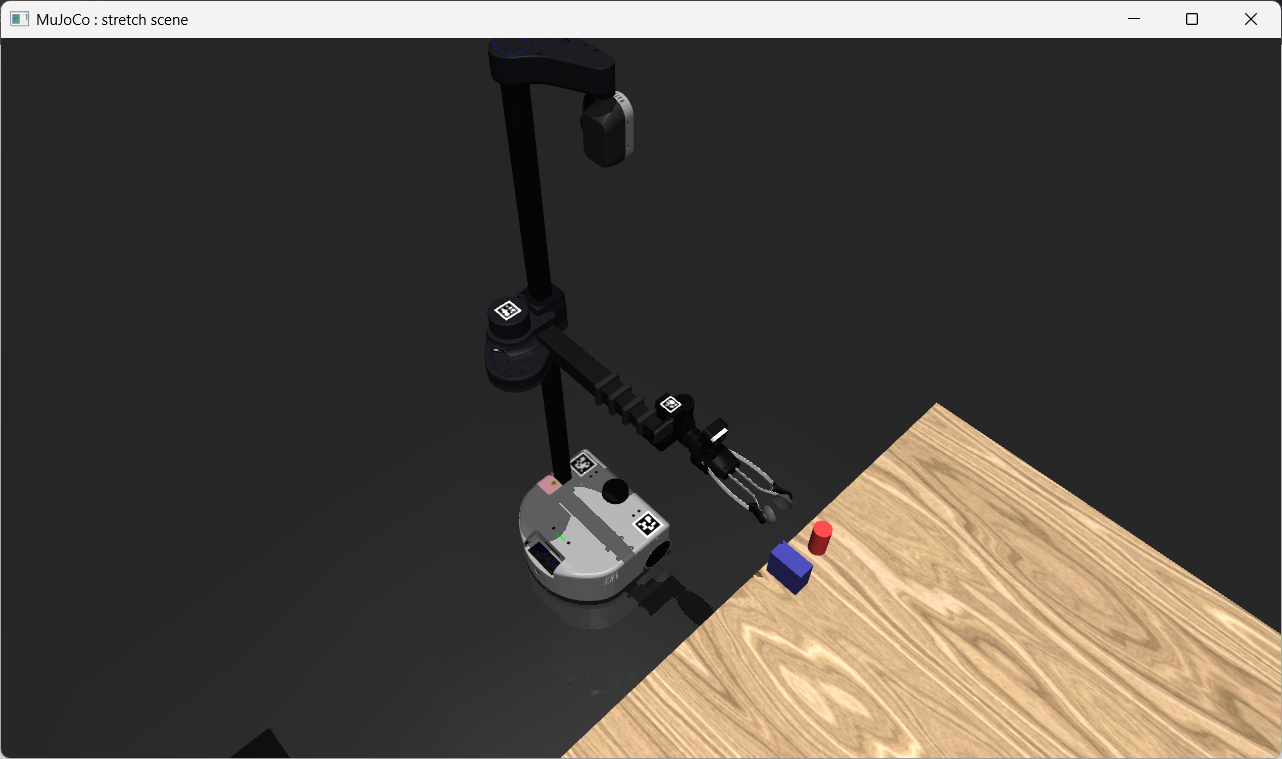
\includegraphics[width=0.5\linewidth]{stretch_sim.png}
    \caption{Default simulation environment}
    \label{fig:base_env}
\end{figure}

Press \textbf{Ctrl+C} to exit.

\section{Part 2: Block Stacking Challenge}

\textbf{Task:} Stack one block on top of the other using teleoperation.

\subsection{Stretch's 9 Degrees of Freedom}

\begin{enumerate}
    \item Base Translation
    \item Base Rotation
    \item Lift
    \item Arm
    \item Wrist Yaw
    \item Wrist Pitch
    \item Wrist Roll
    \item Gripper
    \item Head Pan/Tilt
\end{enumerate}

\subsection{Keyboard Controls}

\begin{table}[H]
\centering
\begin{tabular}{|l|l|}
\hline
\textbf{Keys} & \textbf{Action} \\
\hline
W / S & Base forward/backward \\
D / A & Base rotate right/left \\
Z / X & Lift up/down \\
V / C & Arm extend/retract \\
M / N & Gripper open/close \\
L / J & Wrist yaw \\
U / O & Wrist roll \\
K / I & Wrist pitch \\
H & Toggle head/wrist mode \\
\hline
\end{tabular}
\caption{Primary keyboard mappings (see \texttt{teleop\_mappings.json} for gamepad)}
\end{table}

\begin{figure}[H]
    \centering
    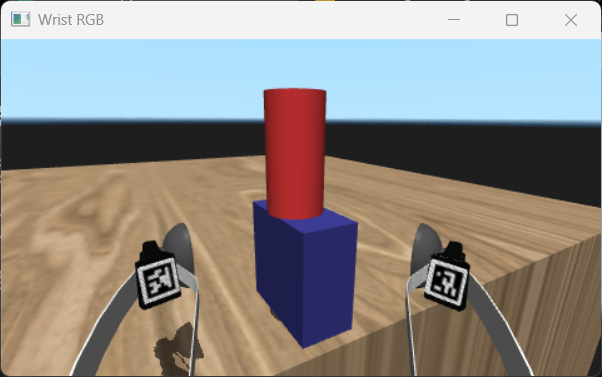
\includegraphics[width=0.5\linewidth]{stacked_blocks.png}
    \caption{Target outcome: one block stacked on top of the other}
    \label{fig:stacked_blocks}
\end{figure}

\textbf{Tips:} Orbit the MuJoCo viewer as needed for better depth perception. Take your time.

\section{Part 3 (Optional): Verify RoboCasa Environment}

This optional step verifies that your computer can run the RoboCasa kitchen environments used in later practices.

Install RoboCasa dependencies:

\begin{lstlisting}[language=bash]
uv pip install -e ".[robocasa]"
uv pip install -e "robocasa@third_party/robocasa"
uv pip install -e "robosuite@third_party/robosuite"
uv run third_party/robosuite/robosuite/scripts/setup_macros.py
uv run third_party/robocasa/robocasa/scripts/setup_macros.py
uv run third_party/robocasa/robocasa/scripts/download_kitchen_assets.py
\end{lstlisting}

\textbf{Note:} Asset download is ~5 GB and takes some time.

Verify \texttt{stretch\_toolkit/robocasa\_config.json} has \texttt{"enabled": true}, then run:

\begin{lstlisting}[language=bash]
uv run teleop_demo.py
\end{lstlisting}

You should see a kitchen environment with cabinets, counters, and appliances.

\begin{figure}[H]
    \centering
    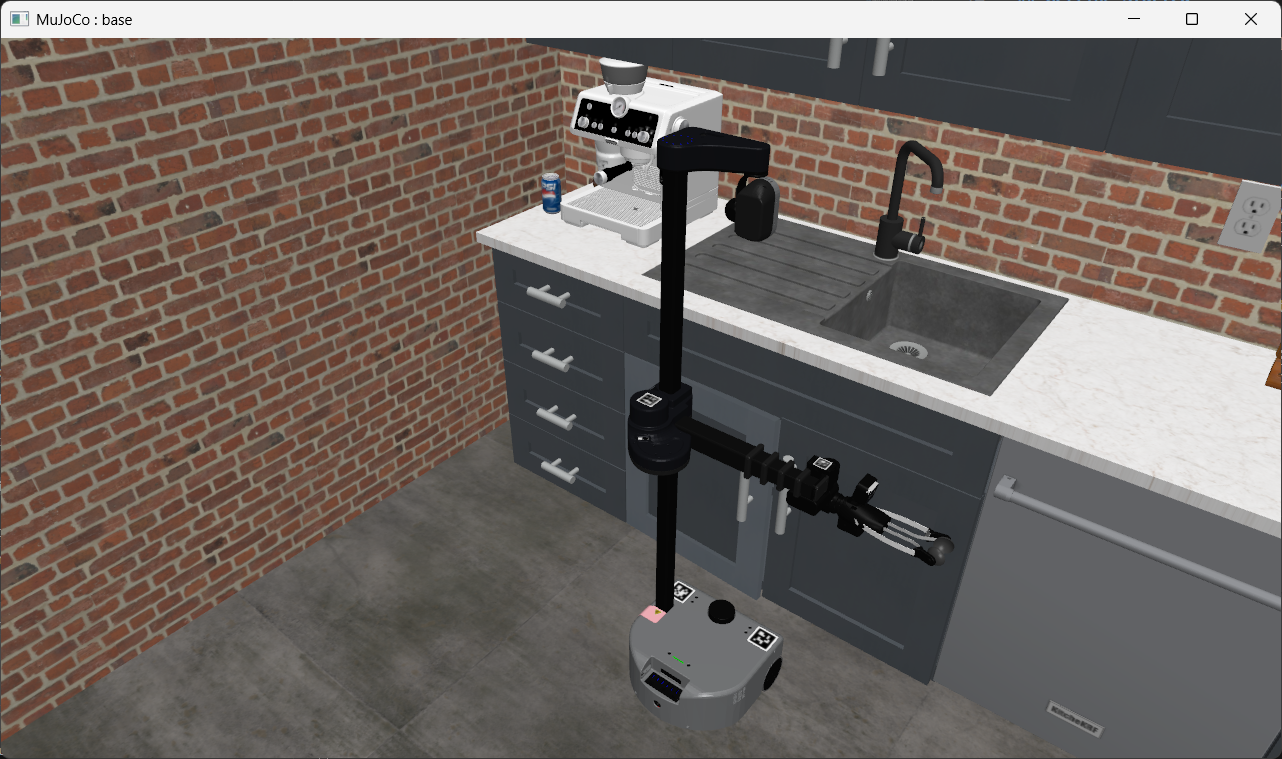
\includegraphics[width=0.5\linewidth]{stretch_robocasa.png}
    \caption{RoboCasa kitchen scene}
    \label{fig:robocasa_env}
\end{figure}

\section{Evidence and Submission}

Submit a PDF report (1-2 pages) containing:

\begin{itemize}
    \item \textbf{Link to a short video:} Move each joint and briefly explain what it does in your own words as it moves.
    \item A screenshot of the stacked blocks result (Part 2).
    \item \textbf{Optional:} A screenshot of the RoboCasa kitchen environment (Part 3).
    \item A short written description of each of the robot's 9 degrees of freedom and its corresponding control key.
\end{itemize}

\textbf{File naming:} \texttt{LastName\_FirstName\_Practice1.pdf}

\section{Troubleshooting}

\textbf{Simulator won't start:} Run \texttt{uv sync} then retry

\textbf{Controls not responding:} Click the MuJoCo viewer window to focus it

\textbf{Physics issues:} Restart simulation with Ctrl+C

\subsection{Resources}

\begin{itemize}
    \item \url{https://github.com/SilentSammy/stretch_mujoco_digital_twin}
    \item \url{https://mujoco.readthedocs.io/}
    \item \url{https://hello-robot.com/stretch-3}
\end{itemize}

\section{Conclusion}

You've installed the Stretch simulator and completed a manipulation task. If you completed the optional section, you also verified the RoboCasa kitchen environment for future practices. Future practices will cover programmatic control, computer vision, and autonomous planning.

Good luck with the block stacking challenge!

\end{document}
